
\section{Performance and Evaluation of Layer-Wise Energy Prediction Models}
\label{sec:results}

\looseness=-1
In the following, we will show how well the predictors for each layer type perform when trained using the \textbf{``layer-wise''} data set (Sec.~\ref{sec:data-collection}), which was divided into three sets: 70\% for training, 20\% for validation, and 10\% for testing. We evaluated models with different feature sets for each layer type (App.~\ref{sec:appendix-feature-sets-experiment}), but chose the best model according to the test $R^2$ score, MSE, and Max-Error. Additionally, we evaluated the 10-fold cross-validation average $R^2$ score and MSE. See Tab.~\ref{tab:layer-modles-performances} for the exact scores and both Fig.~\ref{fig:layer-scatterplots-layers} and Fig.~\ref{fig:layer-scatterplots-activations} for scatter plots.

\looseness=-1
\textbf{Activations.} While often numerous, activations only make up for a small fraction of the model energy consumption (see Fig.~\ref{fig:layer-wise-contribution}). The input features of the Sigmoid, Tanh, and Softmax models are the layer parameters with a polynomial transform of $d=2$ and interaction-only terms. The ReLU model was based solely on MAC count. The models, in the same order, achieved $R^2$ test scores of  0.9905, 0.9761, 0.9913, and 0.9812 respectively. \textbf{Linear.} Compared to activations, Linear layers contribute a significant amount to the total energy needs (1\%-10\%). The predictor uses the MAC count as the only feature and achieved an $R^2$ test score of 0.9992. Other models, based on different feature sets, also performed exceptionally well, but we chose this one for its simplicity. \textbf{MaxPooling.} About as energy-intensive as the Linear layer, the MaxPooling layer is, due to the larger number of possible parameters, more difficult to model. The chosen model uses both standard and log-transformed layer parameters, the MAC count, and polynomial features of $d=2$ to achieve an $R^2$ test score of 0.9995. \textbf{Convolution.} Not only is the Convolutional layer the most energy-expensive of the four (80\%-90\%), but it also has the most configurable parameters, making it the toughest layer to model. Yet surprisingly, the best model uses the MAC count as the only input feature and achieves an $R^2$ test score of 0.9977. App.~\ref{sec:appendix-ablation-analysis} further outlines the importance of the MAC count for this layer.

Given these exceptionally good results, we proceed by testing each predictor's capabilities not on random but real configurations, using the per-layer observations from the \textbf{''model-wise``} data set. As can be seen in Fig.~\ref{fig:layer-preds-real-architectures} the models perform reasonably well: the estimates for the Linear layer are close to perfect ($R^2$ 0.977); the MaxPooling model ($R^2$ 0.559), as well as the Convolutional model ($R^2$ 0.314), overestimate the target considerably; the ReLU model struggles to extrapolate to the new configurations, but fortunately the contribution of these layers to the total energy is negligible. Finally, we sum up all layer-wise estimates for each full architecture measurement in the ``model-wise'' data to evaluate the accuracy of the entire process. The assumption that the sum of layer-wise energy equals total energy consumption holds with negligible differences. (see Fig.~\ref{fig:agg-vs-total-energy}). Fig.~\ref{fig:full-predictions} shows the results of this process. It can be seen that the energy consumption is generally overestimated, resulting in an overall $R^2$ score of 0.352. The scatterplot also indicates that computationally more expensive architectures generally suffer from greater overestimation. Although the models introduced in the previous paragraph showed excellent performance for randomly configured modules, it is evident that the generalization to carefully conceptualized modules from real architectures is not trivial. One reason for this may be the vast set of possible random configurations for the Convolution and MaxPooling layers, of which most are unlikely to appear in the real world. Further experiment showed that integrating even a small additional number of layer configurations derived from actual architectures can result in significant performance improvements (see Sec.~\ref{section:add-real-configs}). Another reason could be that the MAC count not always accurately represents energy consumption due to parallelization and memory optimizations \citep{Dissecting_DBLP:journals/corr/abs-2107-11949, misnomer}.
\begin{table}[t]
    \caption{Performance metrics of the final models that were chosen to model the energy consumption for each layer type.}
    \label{tab:layer-modles-performances}
    \begin{center}
        \begin{tabular}{l|lllll}
        \multicolumn{1}{c}{\bf Module} & \multicolumn{1}{c}{\bf Avg. $R^2$ Cross-Val}  & \multicolumn{1}{c}{\bf Avg. MSE Cross-Val} & \multicolumn{1}{c}{\bf $R^2$ Test Set} & \multicolumn{1}{c}{\bf MSE Test-Set}
        \\ \hline \\
\textbf{Conv2d}     & 0.994 (± 0.005) & -2.291e-05 (± 1.329e-05) & 0.9977 & 2.779e-05  \\
\textbf{MaxPool2d}  & 0.999 (± 0.000) & -2.552e-06 (± 4.612e-06) & 0.9995 & 7.736e-07  \\
\textbf{Linear}     & 0.999 (± 0.000) & -4.284e-05 (± 1.425e-05) & 0.9992 & 3.384e-05  \\
\textbf{ReLU}       & 0.981 (± 0.005) & -1.046e-03 (± 2.284e-04) & 0.9812 & 8.998e-04  \\
\textbf{Sigmoid}    & 0.981 (± 0.008) & -1.047e-03 (± 1.866e-04) & 0.9905 & 7.538e-04  \\
\textbf{Tanh}       & 0.976 (± 0.008) & -1.315e-03 (± 4.252e-04) & 0.9761 & 1.412e-03  \\
\textbf{Softmax}    & 0.989 (± 0.004) & -5.671e-04 (± 1.599e-04) & 0.9913 & 4.972e-04
        \end{tabular}
    \end{center}
\end{table}
\begin{figure}[h]
    \centering
    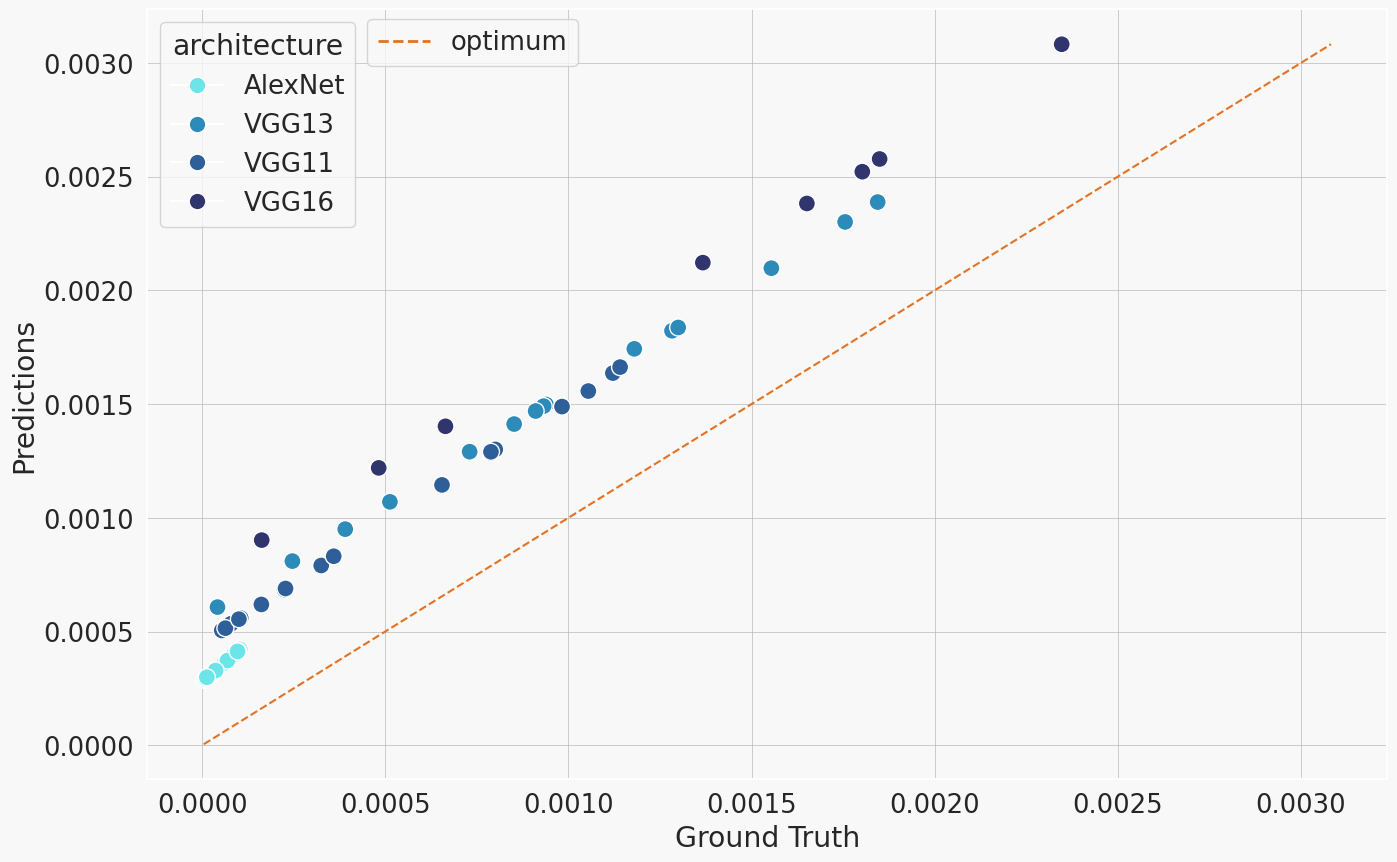
\includegraphics[width=0.85\textwidth]{resources/full-predictions.png}
    \caption{Compares the measured energy consumption and the accumulated predicted energy consumption; the x-axis corresponds to the measured ground truth, the y-axis to the sum of the layer-wise predictions, and the diagonal to the optimal scenario with perfect predictions; overall $R^2$ score: 0.352.}
    \label{fig:full-predictions}
\end{figure}
\begin{figure}[h]
        \centering
        \begin{subfigure}[b]{0.47\textwidth}
            \centering
            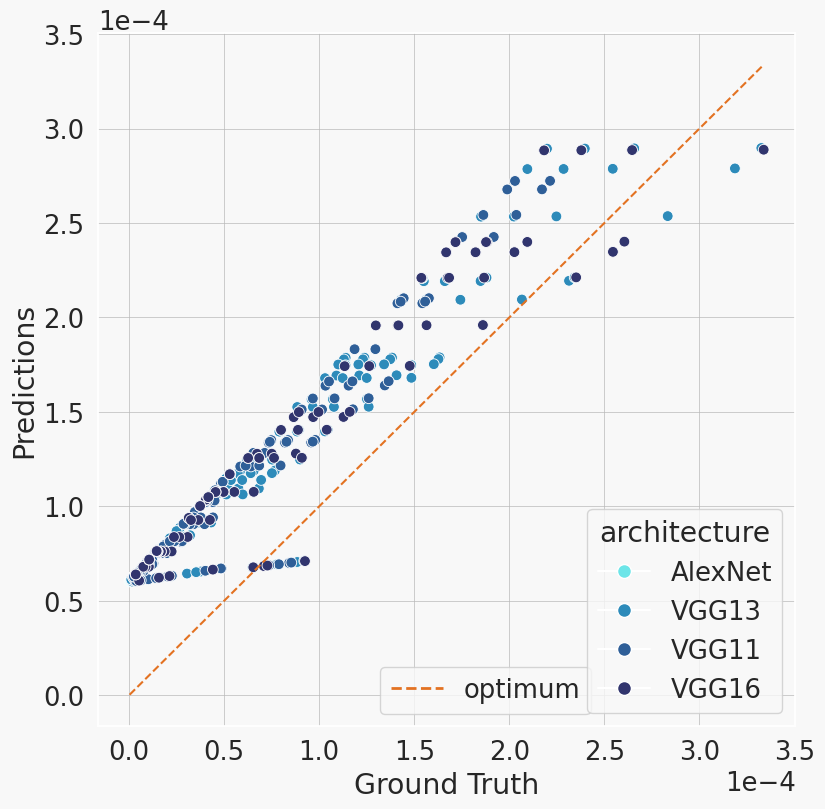
\includegraphics[width=\textwidth]{resources/full-predictions-convolution.png}
            \caption[]%
            {{\small Convolution}}    
            \label{}
        \end{subfigure}
        \hfill
        \begin{subfigure}[b]{0.47\textwidth}  
            \centering 
            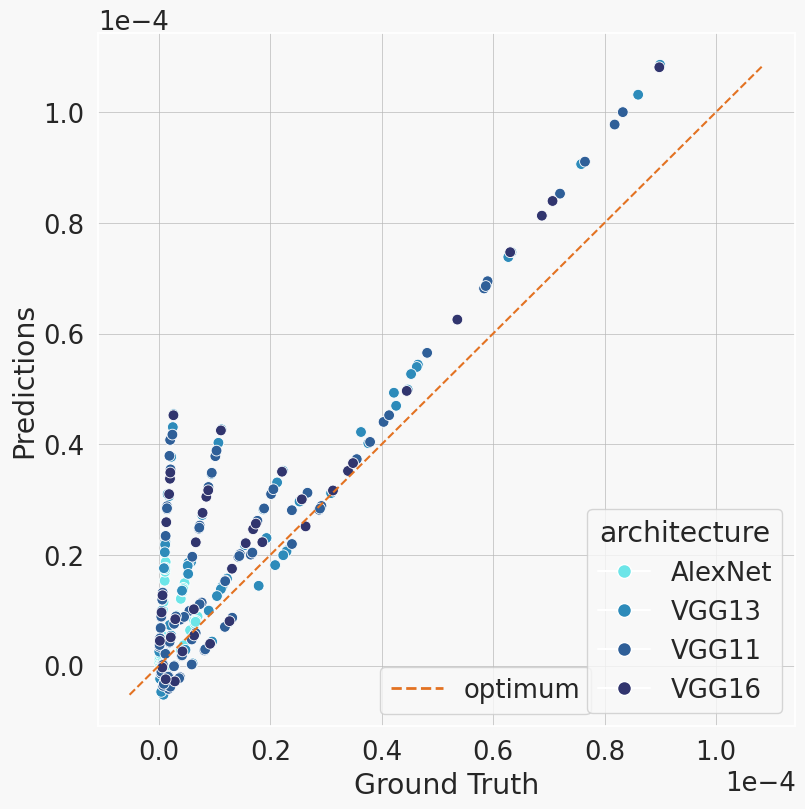
\includegraphics[width=\textwidth]{resources/full-predictions-maxpooling.png}
            \caption[]%
            {{\small MaxPooling}}    
            \label{}
        \end{subfigure}
        \vskip\baselineskip
        \begin{subfigure}[b]{0.47\textwidth}   
            \centering 
            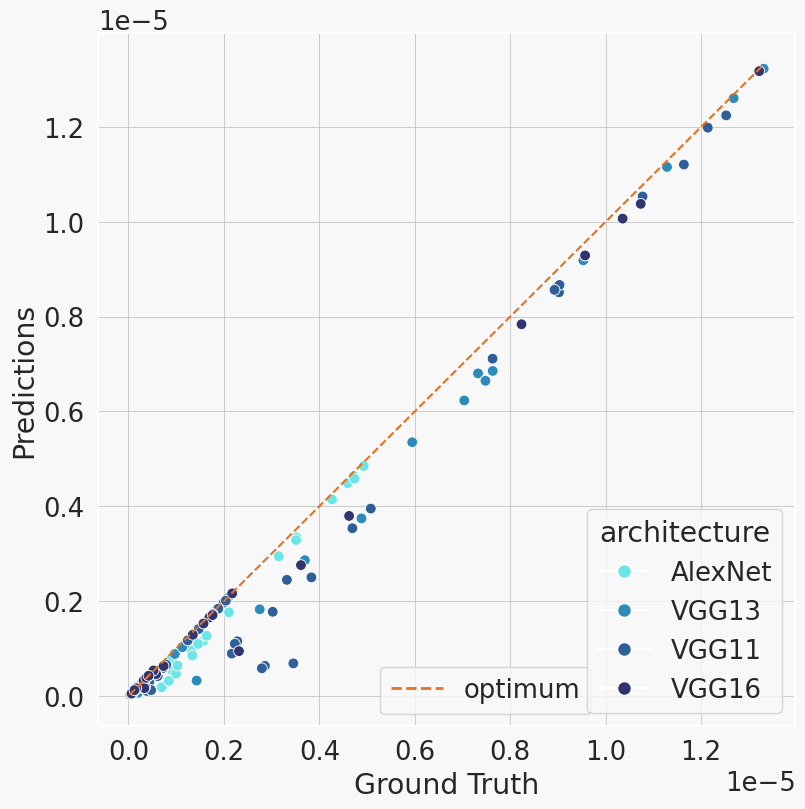
\includegraphics[width=\textwidth]{resources/full-predictions-linear.png}
            \caption[]%
            {{\small Linear}}    
            \label{}
        \end{subfigure}
        \hfill
        \begin{subfigure}[b]{0.47\textwidth}   
            \centering 
            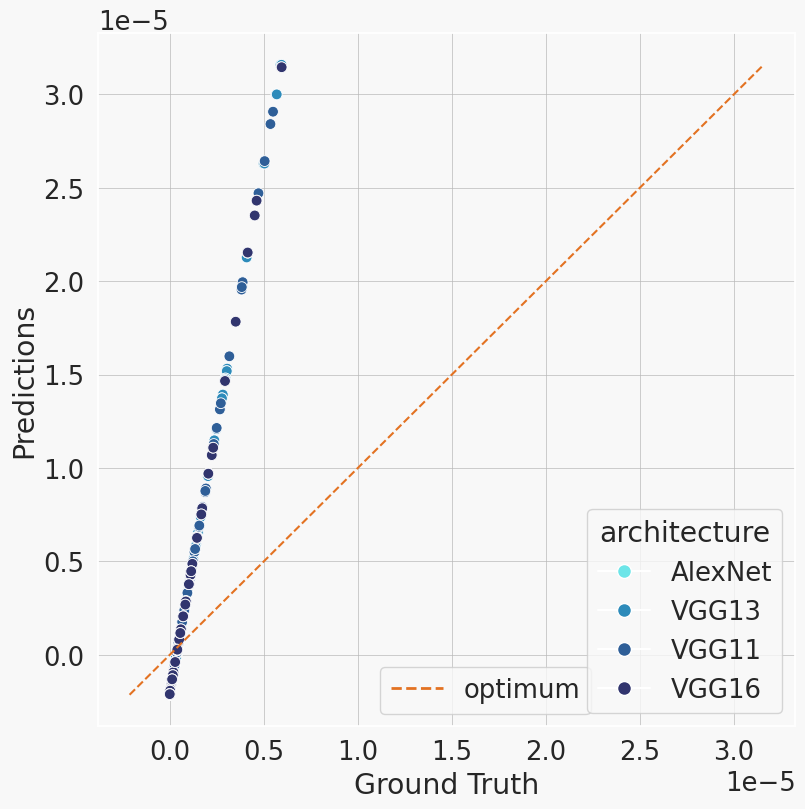
\includegraphics[width=\textwidth]{resources/full-predictions-relu.png}
            \caption[]%
            {{\small ReLU}}    
            \label{}
        \end{subfigure}
        \caption[Shows scatter plots for the layer types in AlexNet and VGG11/13/16, illustrating each model's accuracy when tested on real configurations from these architectures; the x-axis represents the ground truth while the y-axis represents the predicted values, and the diagonal line symbolizes perfect predictions; $R^2$ scores: 0.314 Convolution, 0.559 MaxPooling, 0.977 Linear, -21.51 ReLU.]
        {Shows scatter plots for the layer types in AlexNet and VGG11/13/16, illustrating each model's accuracy when tested on real configurations from these architectures; the x-axis represents the ground truth while the y-axis represents the predicted values, and the diagonal line symbolizes perfect predictions; $R^2$ scores: 0.314 Convolution, 0.559 MaxPooling, 0.977 Linear, -21.51 ReLU.}
        \label{fig:layer-preds-real-architectures}
\end{figure}